\documentclass[conference,letterpaper]{IEEEtran}
\usepackage[T1]{fontenc}
\usepackage{amsmath}
\usepackage{tikz}
\usepackage{pgfplots}
\pgfplotsset{compat=1.18}
\usepackage{url}
\usepackage[hidelinks]{hyperref}
\interdisplaylinepenalty=2500
\title{IntentGuard: Stateful Task-Scoped Authorization for AI Agent Trajectories}
\author{\IEEEauthorblockN{Prabhu Sivapunniyam}\IEEEauthorblockA{Independent Researcher}}
\begin{document}
\maketitle


\begin{abstract}
Tool-using AI agents may propose individually permitted actions whose accumulated effects exceed the user task. Operation allowlists cannot express scoped budgets or required ordering, making this distinction important for repeated access and disclosure. We implement IntentGuard, a trusted runtime that evaluates explicit task contracts against admitted history before executing tools. Its mechanism study isolates per-operation and per-resource budgets, distinct-destination limits, and successful-operation sequences beyond a total action count; it does not claim novelty for counters or finite-state policies themselves. The implementation passes 41 tests. Across 44 synthetic cases with 69 proposals, it matches all expected decisions, executes all 47 authorized proposals, and executes none of 22 proposals requiring blocking or confirmation. A count-only control executes six unauthorized proposals that richer trajectory constraints reject. These results demonstrate deterministic enforcement on constructed inputs, not prompt-injection resistance for a real model, task-completion utility, or superiority over published defenses.
\end{abstract}

\begin{IEEEkeywords}AI agents, task authorization, prompt injection, runtime enforcement, least privilege, trajectory constraints.\end{IEEEkeywords}

\section{Introduction}

An AI assistant retrieving an invoice may possess credentials capable of sending messages, modifying records, and reading unrelated documents. The user may nevertheless have authorized only retrieval of one invoice amount. If retrieved content asks the assistant to forward the invoice externally, a capability check may permit the invocation while the action violates the task. We use authorization drift to describe divergence between task authority and proposed operations or cumulative effects.


Task relevance does not by itself establish authority: sending a document can help resolve an invoice question while violating a recipient restriction. Conversely, an unfamiliar resource can be necessary for a legitimate search. An enforcement system must expose which boundaries are hard constraints and which require confirmation. Treating uncertainty as permission risks disclosure; rejecting every uncertainty can prevent useful work.


IntentGuard evaluates a normalized proposal before execution and returns ALLOW, CONFIRM, or BLOCK with a reason. A trusted tool registry declares required operands and side effects. A task lock serializes authorization, charging, and bounded execution so concurrent calls cannot independently consume the same remaining budget. The human-readable objective is stored but not interpreted semantically; contracts are supplied as structured data to separate enforcement errors from natural-language compilation errors.


The study asks what violations each policy mechanism prevents under matched proposals and what legitimate actions it obstructs. The contribution comprises an executable contract, a guarded in-memory runtime, 21 synthetic pairs, and a reproducible five-policy comparison. The results isolate static boundaries, scoped budgets, and ordered execution. The planner proposes; the trusted runtime authorizes. A full agent study remains necessary for adaptive attacks, ambiguous tasks, and generalization beyond the selected inputs.


\section{Related Work and Research Gap}

\subsection{Evaluation and task alignment}

AgentDojo \cite{ref1} and InjecAgent \cite{ref2} provide environments for studying indirect prompt injection and tool-using agents. Their scope is broader than the fixed proposals used here; percentages from these datasets cannot be ranked against our diagnostic counts. Task Shield \cite{ref3} checks whether instructions and calls contribute to the user task. This overlaps with a proposed semantic layer, whereas the present design exposes deterministic constraints for independent inspection and replay.


\subsection{Authorization, provenance, and trajectories}

DRIFT \cite{ref4} combines a planned function trajectory, parameter constraints, dynamic validation, and instruction isolation. IntentGuard enforces explicit budgets and a fixed operation sequence, not equivalent plan reasoning or memory isolation. PAuth \cite{ref5} derives task-scoped specifications and binds values to signed provenance; it directly addresses operator permission versus authority for a concrete operation. IntentGuard neither originates task-scoped authorization nor provides PAuth's provenance guarantee. CaMeL \cite{ref6} separates control and data flows and constrains tool calls through capabilities. Explicit resource and destination sets alone cannot provide its information-flow guarantees.


These approaches already address task alignment, authorization, provenance, or trajectories. We do not assert that none addresses stateful authorization. The gap examined here is an ablation question: under identical tool semantics and proposals, which explicit history constraints reject violations that a total count permits? A resource may be accessed too often while the global budget remains available, and a send may occur before a required draft. Published defenses are contextual comparisons, not implemented baselines; assessing incremental research novelty requires faithful external comparisons.


\section{System Model and Methodology}

\subsection{Trust boundary and representation}

The model contains a user, an untrusted or fallible planner, a trusted contract authority, a guarded runtime, and bounded tools. The host owns the runtime and tool credentials. The planner supplies proposals, not contract updates, approvals, or history. Attacker-controlled tool content and planner mistakes are in scope; compromise of the host, runtime, or tool adapter is excluded. All evaluated effects are synthetic and remain in memory.


Let C = (O, R, D, P, F, K) denote allowed operations, resources, destinations, prohibited operations, confirmation-required effects, and an optional count limit. A proposal a = (o, r, d, s) contains operation, resource, optional destination, and optional effect. The runtime validates operands and derives s from trusted tool metadata. Extend C with operation budgets B\_o, resource budgets B\_r, an optional ordered sequence Q, and a distinct-destination bound U. State H stores admitted counts, destination set, and the successful sequence index. Counts include failed invocations; sequence progress does not. Hard constraints are evaluated before confirmation; only ALLOW reaches a tool.


\subsection{Worked task contract}

Consider: "Read invoice 123. Ask before sending it to me. Do not access other documents." Listing 1 encodes this task with a two-invocation budget. The registered send adapter requires a destination and declares external\_communication. Omitting that effect from the proposal cannot suppress confirmation.


\begin{center}
\begin{minipage}{\columnwidth}
\scriptsize\textbf{Listing 1. Worked task contract}
\begin{verbatim}
{
  "objective": "Read invoice; confirm sending",
  "allowed_operations": ["read", "send"],
  "allowed_resources": ["invoice_123"],
  "allowed_destinations": ["user@example.com"],
  "prohibited_operations": ["delete"],
  "confirmation_required": ["external_communication"],
  "max_action_count": 2
}
\end{verbatim}
\end{minipage}
\end{center}


\begin{table}[ht]
\caption{Worked contract outcomes}\centering\scriptsize
\begin{tabular}{p{.53\columnwidth}cc}\hline
Separate proposal & History h & Decision \\
Read invoice\_123 & 0 & ALLOW \\
Read payroll & 0 & BLOCK \\
Send to external address & 0 & BLOCK \\
Send to user@example.com & 0 & CONFIRM \\
Read invoice\_123 & 2 & BLOCK \\\hline
\end{tabular}\end{table}


Table I treats each row as a separate proposal. Rows other than the exhausted-budget example begin at h = 0; the last row begins after two admitted reads. The contract authorizes read attempts but does not automatically approve sending. A valid recipient yields CONFIRM, whereas an external recipient violates a hard boundary and yields BLOCK. CONFIRM suspends execution; authenticated approval and resumption are not implemented.


\section{Architecture and Authorization Algorithm}

\subsection{Guarded execution boundary}

Figure 1 distinguishes the proposed compilation stage from implemented enforcement. Natural-language intent would be compiled and validated by the host or user before installation. Current experiments supply structured contracts manually. Validated frozen objects are immutable data, not signed authority. The trusted registry and task lock mediate proposals against runtime-owned history. A process boundary remains necessary if planner code itself is adversarial.


\begin{figure}[ht]
\centering
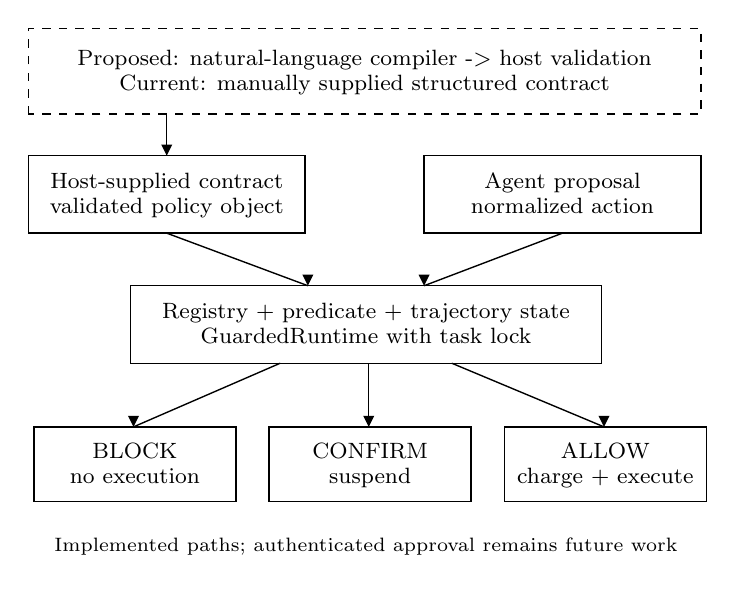
\begin{tikzpicture}[x=1pt,y=1pt]
\draw[line width=.5pt,dashed] (4,164) rectangle (247,195);
\node[anchor=base,font=\fontsize{8}{9}\selectfont] at (125.5,181.5) {Proposed: natural-language compiler -\textgreater{} host validation};
\node[anchor=base,font=\fontsize{8}{9}\selectfont] at (125.5,172.5) {Current: manually supplied structured contract};
\draw[line width=.5pt] (54,164) -- (54,149);
\fill (54,149) -- (52,153) -- (56,153) -- cycle;
\draw[line width=.5pt] (4,121) rectangle (104,149);
\node[anchor=base,font=\fontsize{8}{9}\selectfont] at (54.0,137.0) {Host-supplied contract};
\node[anchor=base,font=\fontsize{8}{9}\selectfont] at (54.0,128.0) {validated policy object};
\draw[line width=.5pt] (147,121) rectangle (247,149);
\node[anchor=base,font=\fontsize{8}{9}\selectfont] at (197.0,137.0) {Agent proposal};
\node[anchor=base,font=\fontsize{8}{9}\selectfont] at (197.0,128.0) {normalized action};
\draw[line width=.5pt] (41,74) rectangle (211,102);
\node[anchor=base,font=\fontsize{8}{9}\selectfont] at (126.0,90.0) {Registry + predicate + trajectory state};
\node[anchor=base,font=\fontsize{8}{9}\selectfont] at (126.0,81.0) {GuardedRuntime with task lock};
\draw[line width=.5pt] (54,121) -- (105,102);
\fill (105,102) -- (103,106) -- (107,106) -- cycle;
\draw[line width=.5pt] (197,121) -- (147,102);
\fill (147,102) -- (145,106) -- (149,106) -- cycle;
\draw[line width=.5pt] (6,24) rectangle (79,51);
\node[anchor=base,font=\fontsize{8}{9}\selectfont] at (42.5,39.5) {BLOCK};
\node[anchor=base,font=\fontsize{8}{9}\selectfont] at (42.5,30.5) {no execution};
\draw[line width=.5pt] (91,24) rectangle (164,51);
\node[anchor=base,font=\fontsize{8}{9}\selectfont] at (127.5,39.5) {CONFIRM};
\node[anchor=base,font=\fontsize{8}{9}\selectfont] at (127.5,30.5) {suspend};
\draw[line width=.5pt] (176,24) rectangle (249,51);
\node[anchor=base,font=\fontsize{8}{9}\selectfont] at (212.5,39.5) {ALLOW};
\node[anchor=base,font=\fontsize{8}{9}\selectfont] at (212.5,30.5) {charge + execute};
\draw[line width=.5pt] (95,74) -- (42,51);
\fill (42,51) -- (40,55) -- (44,55) -- cycle;
\draw[line width=.5pt] (127,74) -- (127,51);
\fill (127,51) -- (125,55) -- (129,55) -- cycle;
\draw[line width=.5pt] (157,74) -- (212,51);
\fill (212,51) -- (210,55) -- (214,55) -- cycle;
\node[anchor=base,font=\fontsize{7}{9}\selectfont] at (126,6) {Implemented paths; authenticated approval remains future work};
\end{tikzpicture}
\caption{Proposed compilation (dashed) and implemented execution boundary. Trusted registry metadata and a task lock mediate mock tools. CONFIRM suspends; authenticated approval and resumption remain future work.}
\end{figure}


The wrapper rejects unknown adapters, missing required destinations, unexpected destination fields, and conflicting side-effect declarations. It derives omitted effects from trusted metadata before calling the predicate. Explicitly prohibited operations take precedence over an allowlist entry. Operation, resource, destination, budget, and sequence violations take precedence over confirmation. Figure 2 summarizes the resulting decision flow.


\subsection{Execution algorithm}

Every ALLOW charges global, operation, and resource counts and records its destination before the handler runs. Only a successful handler advances the sequence; reentrant execution is rejected. A tool exception is retained in the result and does not refund the charge. BLOCK and CONFIRM produce trace records without tool execution or history consumption. Malformed contracts and proposals raise validation errors before execution. Decision and outcome traces are neither durable nor tamper-evident.


\begin{figure}[ht]
\centering
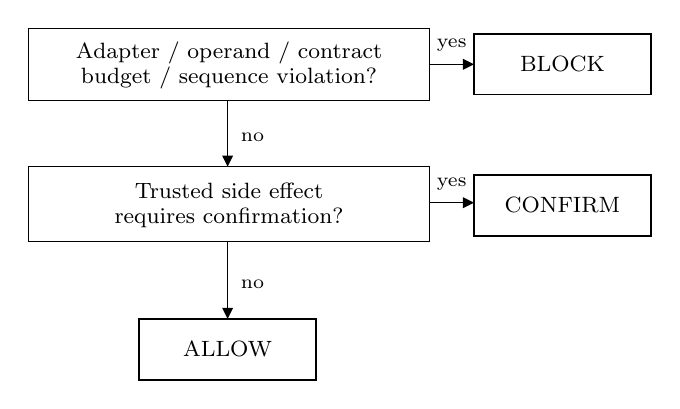
\begin{tikzpicture}[x=1pt,y=1pt]
\draw[line width=.5pt] (22,113) rectangle (167,139);
\node[anchor=base,font=\fontsize{8}{9}\selectfont] at (94.5,128.0) {Adapter / operand / contract};
\node[anchor=base,font=\fontsize{8}{9}\selectfont] at (94.5,119.0) {budget / sequence violation?};
\draw[line width=.5pt] (183,115) rectangle (247,137);
\node[anchor=base,font=\fontsize{8}{9}\selectfont] at (215.0,123.5) {BLOCK};
\draw[line width=.5pt] (167,126) -- (183,126);
\fill (183,126) -- (179,124) -- (179,128) -- cycle;
\node[anchor=base,font=\fontsize{7}{9}\selectfont] at (175,132) {yes};
\draw[line width=.5pt] (22,62) rectangle (167,89);
\node[anchor=base,font=\fontsize{8}{9}\selectfont] at (94.5,77.5) {Trusted side effect};
\node[anchor=base,font=\fontsize{8}{9}\selectfont] at (94.5,68.5) {requires confirmation?};
\draw[line width=.5pt] (94,113) -- (94,89);
\fill (94,89) -- (92,93) -- (96,93) -- cycle;
\node[anchor=base,font=\fontsize{7}{9}\selectfont] at (103,98) {no};
\draw[line width=.5pt] (183,64) rectangle (247,86);
\node[anchor=base,font=\fontsize{8}{9}\selectfont] at (215.0,72.5) {CONFIRM};
\draw[line width=.5pt] (167,76) -- (183,76);
\fill (183,76) -- (179,74) -- (179,78) -- cycle;
\node[anchor=base,font=\fontsize{7}{9}\selectfont] at (175,82) {yes};
\draw[line width=.5pt] (62,12) rectangle (126,34);
\node[anchor=base,font=\fontsize{8}{9}\selectfont] at (94.0,20.5) {ALLOW};
\draw[line width=.5pt] (94,62) -- (94,34);
\fill (94,34) -- (92,38) -- (96,38) -- cycle;
\node[anchor=base,font=\fontsize{7}{9}\selectfont] at (103,45) {no};
\end{tikzpicture}
\caption{Runtime decision flow after proposal validation. Missing required destinations and hard violations block before confirmation; side effects come from trusted metadata.}
\end{figure}


\begin{center}
\begin{minipage}{.98\columnwidth}
\small\textbf{Algorithm 1. Guarded execution}\par
Input: contract C, proposal a, trusted registry T\par
State: counts, destinations, sequence index; lock L\par
1  Validate proposal; acquire L; reject reentrancy\par
2  Derive effects and validate adapter operands\par
3  Check static boundaries and global count\par
4  Check operation/resource budgets, destinations,\par
     and next successful-sequence operation\par
5  Apply confirmation after hard constraints\par
6  If BLOCK or CONFIRM: trace; return\par
7  Charge all budgets; record destination\par
8  Execute handler; retain result or exception\par
9  Advance sequence only if handler succeeds\par
10 Trace outcome; release L on every exit\par
\end{minipage}
\end{center}


\subsection{Cumulative safety and concurrency}

For a finite limit K and an initial count of zero, every admission requires h \textless{} K and increments h before invoking a handler. Since one task lock serializes this transition, induction bounds admitted invocations by K, including failed invocations. The same argument applies to each scoped budget. Under the lock, an admitted operation must equal the next sequence symbol; success advances exactly one position. This property assumes a trusted host and a shared runtime instance. It does not extend to independent processes with separate counters, direct tool calls that bypass the wrapper, or authenticated multi-agent delegation.


The implementation holds the lock across bounded mock execution. This simplifies accounting and prevents a check-then-execute race, but can serialize slow handlers in a deployment. A future reservation-based scheduler must preserve the same count invariant while handling cancellation, retries, and persistence. Confirmation similarly needs a trusted approval record bound to the task, operands, and contract version; a planner-supplied approval flag is not accepted.


\section{Experimental Evaluation}

\subsection{Cases and local controls}

The benchmark retains 15 paired designs P01-P15 and two original fixtures, and adds six trajectory pairs T01-T06. The resulting 44 cases contain 69 proposals: 47 ALLOW, 20 BLOCK, and two CONFIRM. New pairs isolate repeated resource access, repeated sends, ordering, destination cardinality, cross-operation resource use, and replay after sequence completion. Each drift member stays within its total count. Labels are authored before execution, without independent review.


Five policies receive the same proposals and trusted tool metadata. No enforcement removes task restrictions. Operation only retains the operation allowlist. No history retains static boundaries and confirmation but removes all history constraints. Count only adds the global count while omitting richer trajectory policy. IntentGuard enables every constraint. These local controls isolate mechanisms; they do not reproduce Task Shield, DRIFT, PAuth, or CaMeL.


Each case starts with a fresh runtime and zero charged actions. Its complete proposal sequence is replayed, including proposals following a denial. Handlers append synthetic effects to an in-memory list; no files, messages, or financial systems are changed. The original injection fixture's untrusted text is metadata, not input to an LLM. Consequently, the study evaluates fixed action proposals, not whether an attack successfully induces a model to generate them.


\subsection{Outcomes and implementation verification}

We count decisions matching the predefined labels, cases with every decision correct, and authorized versus unauthorized mock executions. A proposal labeled CONFIRM is considered unauthorized to execute before approval. Authorized execution measures whether the mock handler was called for an ALLOW-labeled proposal; it does not measure completion of a user's natural-language task. Baseline disagreements are retained as results rather than treated as runner failures.


The 41-test suite covers the original deterministic checks, input validation, destination and confirmation behavior, hard-block precedence, execution suppression, failed-call accounting, concurrency, and benchmark-runner regressions. A concurrency test submits 40 calls through eight worker threads to one runtime with a limit of two. Additional tests exercise scoped budgets, ordered success, failed-step accounting, distinct destinations, replay rejection, reentrancy, immutable history, and concurrent operation-budget admission. Tests also verify that omitted side effects cannot bypass confirmation and incorrect benchmark labels cause a nonzero runner exit.


\subsection{Whole-runtime timing protocol}

Each measured workflow performs three mock calls: read, draft, and send. Conditions include direct handlers, a static contract runtime with a total count, and full trajectory runtimes with 1, 10, 100, 1,000, or 10,000 allowed resources. Contracts and proposals are preconstructed; runtime initialization, operand checks, locking, history, traces, and mock execution are timed together. This is local workflow latency, not model inference or network latency.


Each condition receives 100 warmups and 2,000 measured workflows. Condition order is shuffled each round with seed 20261002. We report linearly interpolated p50, p95, and p99 workflow latency. The 14,000 measured workflows comprise 42,000 calls, not independent security cases. Measurements were collected October 2, 2026, using CPython 3.12.14 on Windows 11 build 26200, Intel64 Family 6 Model 189. Background activity was not isolated; tail comparisons are descriptive.


\subsection{Reproduction and evidence retention}

The runner retains expected and actual decisions, effects, and normalized UTF-8 source hashes. This revision uses trajectory\_benchmark\_results.json and workflow\_timing\_results.json, including raw workflow samples. The earlier predicate snapshots remain historical evidence and do not support the new runtime measurements. Tests and benchmark execution are configured for continuous integration. No statistical significance or population-level attack-success claim follows from these fixed cases.


\section{Results and Analysis}

\subsection{Benefits observed in fixed-proposal replay}

All 41 automated tests pass. IntentGuard matches 69/69 decisions across 44 cases, executes 47/47 authorized proposals, blocks 20 proposals, and suspends two for confirmation. Table II reports decision agreement, unauthorized execution, and authorized execution. No policy reports mock tool errors.


\begin{table}[ht]
\caption{Decision agreement and mock executions}\centering\scriptsize
\begin{tabular}{lccc}\hline
Policy & Agreement & Unauth. & Auth. \\
No guard & 47/69 & 22 & 47/47 \\
Operation only & 52/69 & 17 & 47/47 \\
No history & 62/69 & 7 & 47/47 \\
Count only & 63/69 & 6 & 47/47 \\
IntentGuard & 69/69 & 0 & 47/47 \\\hline
\end{tabular}\end{table}


\begin{figure}[ht]
\centering
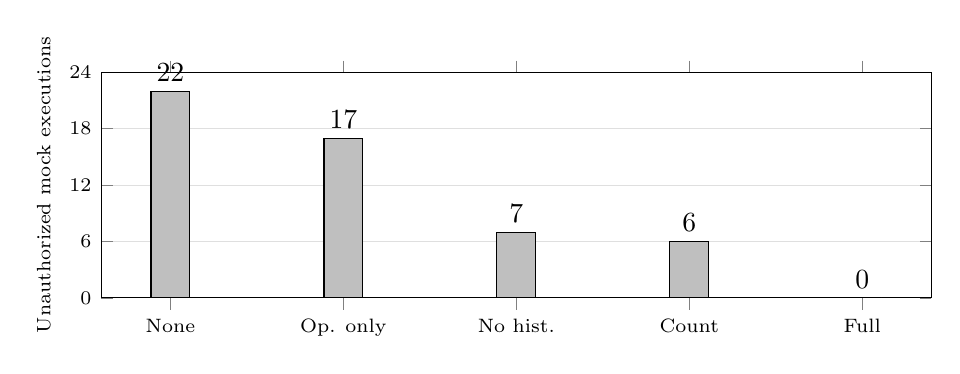
\begin{tikzpicture}
\begin{axis}[width=\columnwidth,height=1.75in,scale only axis=false,tick label style={font=\scriptsize},label style={font=\scriptsize},ymajorgrids=true,grid style={gray!25},ymin=0,ymax=24,ytick={0,6,12,18,24},ylabel={Unauthorized mock executions},symbolic x coords={None,Op. only,No hist.,Count,Full},xtick=data,ybar,bar width=14pt,nodes near coords,]
\addplot[fill=gray!50,draw=black] coordinates {(None,22) (Op. only,17) (No hist.,7) (Count,6) (Full,0)};
\end{axis}
\end{tikzpicture}
\caption{Unauthorized mock executions among 22 BLOCK- or CONFIRM-labeled proposals. Full denotes IntentGuard. All policies execute the same 47 authorized proposals.}
\end{figure}


The full policy prevents 17 unauthorized executions admitted by operation-only enforcement. No-history admits seven; count-only admits six. Those six distinguish richer state from a total counter: repeated resource access, repeated sends, premature send, a second destination, cross-operation access, and a completed-sequence replay. All controls preserve the same 47 authorized proposals. This is mechanism coverage on authored cases, not independent evidence of broad robustness.


\subsection{Whole-runtime cost}

For one allowed resource, the full three-call workflow has p50/p95/p99 latency of 17.9/26.6/45.9 microseconds, versus 16.4/24.9/52.0 for the static runtime and 0.4/0.6/0.8 for direct handlers. The difference in medians is 1.5 microseconds between full and static conditions; the reversed p99 ordering does not establish an advantage.


\begin{figure}[ht]
\centering
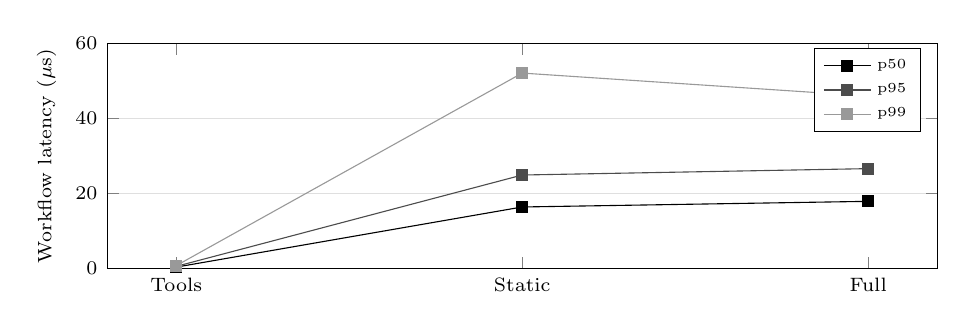
\begin{tikzpicture}
\begin{axis}[width=\columnwidth,height=1.75in,scale only axis=false,tick label style={font=\scriptsize},label style={font=\scriptsize},ymajorgrids=true,grid style={gray!25},ymin=0,ymax=60,ytick={0,20,40,60},ylabel={Workflow latency ($\mu$s)},legend style={font=\tiny},xtick={1,2,3},xticklabels={Tools,Static,Full},]
\addplot[black,mark=square*] coordinates {(1,0.4) (2,16.4) (3,17.9)};\addlegendentry{p50}\addplot[black!70,mark=square*] coordinates {(1,0.6) (2,24.904999999999994) (3,26.604999999999997)};\addlegendentry{p95}\addplot[black!40,mark=square*] coordinates {(1,0.8) (2,52.03299999999997) (3,45.93099999999997)};\addlegendentry{p99}
\end{axis}
\end{tikzpicture}
\caption{Local three-call workflow percentiles over 2,000 samples per condition: p50 (black), p95 (dark gray), p99 (light gray). No LLM or network is involved.}
\end{figure}


\subsection{Resource scaling and interpretation}

Across 1-10,000 allowed resources, full-runtime p50 spans 17.9-18.0 microseconds and p95 spans 26.3-27.4. No monotonic increase appears. Policy construction is excluded, and the workload uses one resource, short histories, and immediate handlers. These results cannot predict large-history or distributed-system cost.


\begin{figure}[ht]
\centering
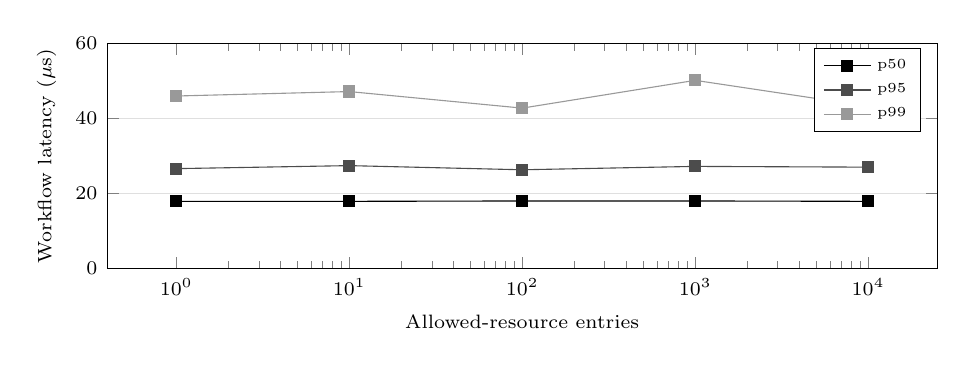
\begin{tikzpicture}
\begin{axis}[width=\columnwidth,height=1.75in,scale only axis=false,tick label style={font=\scriptsize},label style={font=\scriptsize},ymajorgrids=true,grid style={gray!25},ymin=0,ymax=60,ytick={0,20,40,60},ylabel={Workflow latency ($\mu$s)},legend style={font=\tiny},xlabel={Allowed-resource entries},xmode=log,xtick={1,10,100,1000,10000},]
\addplot[black,mark=square*] coordinates {(1,17.9) (10,17.9) (100,18.0) (1000,18.0) (10000,17.9)};\addlegendentry{p50}\addplot[black!70,mark=square*] coordinates {(1,26.604999999999997) (10,27.404999999999994) (100,26.3) (1000,27.2) (10000,27.0)};\addlegendentry{p95}\addplot[black!40,mark=square*] coordinates {(1,45.93099999999997) (10,47.11199999999999) (100,42.708) (1000,50.1) (10000,43.201)};\addlegendentry{p99}
\end{axis}
\end{tikzpicture}
\caption{Whole-runtime resource-set scaling, with p50 (black), p95 (dark gray), and p99 (light gray). Contracts are preconstructed; histories remain short.}
\end{figure}


No iterative optimizer is used, so a convergence claim would be inapplicable. The figures instead report latency percentiles and scaling. Real agent completion, attack success, confirmation burden, token usage, and model-loop latency remain unmeasured.


\section{Limitations}

\subsection{Evidence and construct validity}

The 44 cases exercise known mechanisms and are not a random or held-out task sample. Labels have not received independent review, and no adaptive attacker or LLM generates proposals. The paired cases explain why particular predicates matter, but a perfect result does not establish population-level precision, recall, or attack success. Preserving 47 authorized mock executions is not evidence of natural-language task completion.


The controls are deliberately limited. Operation-only enforcement cannot inspect resources or recipients, and count-only enforcement cannot express scoped budgets or ordering. Their failures on such inputs follow from their definitions. These comparisons isolate mechanisms, not a state-of-the-art ranking. Future studies must include realistic discovery tasks where strict resource enumeration can block legitimate work, along with ambiguous requests and independently reproduced published defenses.


\subsection{Trust and implementation boundary}

Contracts are supplied by the experimenter, avoiding natural-language ambiguity and compilation errors. The guarded runtime owns trajectory state and a tool registry within one process, but does not authenticate users, persist state, isolate malicious Python code, or prevent a compromised host from invoking tools directly. Frozen dataclasses and a lock are implementation mechanisms, not cryptographic or operating-system security boundaries.


The registry defines destination requirements and effects for each supported adapter. Incorrect metadata or an adapter that uses undeclared operands can invalidate enforcement. Pure predicate calls outside the wrapper still rely on caller-supplied history and action fields. CONFIRM suspends execution but cannot currently accept and authenticate a user's approval. Durable, operand-bound approval and contract updates remain necessary for a complete interactive workflow.


\subsection{Measurement and generalization}

The runtime measurement covers a three-call authorized path on one machine with preconstructed contracts. Interpreter behavior, caches, scheduling, and background load influence its percentiles. The concurrency test verifies a count property for one scenario; it is not a concurrency performance benchmark. Broader measurements should vary action mix, misses, key lengths, policy construction, logging, persistence, and handler latency, reporting tail and end-to-end costs separately.


Resource budgets count admitted calls across operations, not bytes or aggregate value. A destination-cardinality bound does not track data composition, and a fixed sequence is not semantic plan verification. No semantic judge, provenance system, aggregate-value budget, disclosure-composition policy, or authenticated delegation mechanism is evaluated. The remaining P16-P20 designs require these additional capabilities. The system therefore cannot claim protection against general information-flow attacks, cross-agent authority laundering, or arbitrary multi-step prompt injection. Statistical claims require appropriately sampled tasks and a justified analysis, not additional repetitions of fixed deterministic inputs.


\section{Conclusion and Future Work}

IntentGuard enforces explicit task authority against admitted history. It passes 41 tests and matches 69/69 decisions on 44 synthetic cases, preserving 47 authorized executions with zero unauthorized executions. Six drift trajectories remain admissible under a total count but are rejected by scoped budgets, destination cardinality, or successful-operation ordering. This supports a deterministic mechanism claim.


The next study should use 50 distinct tasks with benign and injected contexts, yielding 100 task-context conditions, and real model-generated proposals. This is a proposed study, not a completed experiment. Compilation errors must be evaluated separately, labels independently reviewed, and published baselines faithfully reproduced under matched tool and attack budgets. Authenticated approvals must bind task, exact operands, and contract version, with single-use redemption, expiration, substitution, and concurrency tests. Meaningful novelty and practical agent benefit remain to be demonstrated.


\begin{thebibliography}{00}

\bibitem{ref1} E. Debenedetti, J. Zhang, M. Balunovic, L. Beurer-Kellner, M. Fischer, and F. Tramer, "AgentDojo: A Dynamic Environment to Evaluate Prompt Injection Attacks and Defenses for LLM Agents," in Advances in Neural Information Processing Systems, vol. 37, 2024. doi: 10.52202/079017-2636.

\bibitem{ref2} Q. Zhan, Z. Liang, Z. Ying, and D. Kang, "InjecAgent: Benchmarking Indirect Prompt Injections in Tool-Integrated Large Language Model Agents," in Findings of ACL, 2024, pp. 10471-10506. doi: 10.18653/v1/2024.findings-acl.624.

\bibitem{ref3} F. Jia, T. Wu, X. Qin, and A. Squicciarini, "The Task Shield: Enforcing Task Alignment to Defend Against Indirect Prompt Injection in LLM Agents," in Proc. ACL, 2025, pp. 29680-29697. doi: 10.18653/v1/2025.acl-long.1435.

\bibitem{ref4} H. Li, X. Liu, H.-C. Chiu, D. Li, N. Zhang, and C. Xiao, "DRIFT: Dynamic Rule-Based Defense with Injection Isolation for Securing LLM Agents," in Advances in Neural Information Processing Systems, vol. 38, 2025. doi: 10.52202/085713-2791.

\bibitem{ref5} R. K. Sharma, L. Jiang, S. Chen, and Z. Lin, "Beyond OAuth: Task-Scoped Authorization for AI Agents via Natural Language Slices," arXiv:2603.17170v2, Aug. 2026. doi: 10.48550/arXiv.2603.17170.

\bibitem{ref6} E. Debenedetti et al., "Defeating Prompt Injections by Design," arXiv:2503.18813v2, Jun. 2025. doi: 10.48550/arXiv.2503.18813.

\end{thebibliography}

\end{document}
